


\paragraph{Research Team}
Prof. Dr. rer. nat. Brigitte M. Kudielka (Professor of Health Psychology), Dr. rer. nat. Silja Bellingrath (Postdoctoral Fellow, Health Psychology), Dipl. Psych. Nicolas Feuerhahn (Doctoral Student/Research Associate, Health Psychology).

\subsubsection{Health Psychology}

Stress is a common condition of human life, and stress is significantly involved in the maintenance of health or the development of disease. The health psychology research group is mainly interested in the phenomenon of stress and its acute psychological and biological effects, as well as its long-term consequences on human health and well-being. The main endocrine stress systems of the body are the sympathetic-adrenal-medullary-axis (SAM) and the hypothalamic-pituitary-adrenal (HPA) axis; these trigger the release of catecholamines (adrenaline and noradrenaline) from the adrenal medulla and glucocorticoids (e.g. cortisol) from the adrenal cortex (see Kudielka \& Kirschbaum, 2007; Kudielka \& W�st, in press). The release of stress-related hormones supports the adaptation process of the organism to changes and can protect the body in the short run. In contrast, the bodily responses to stress can cause damage in the long run, and can eventually promote the development of several stress-related diseases. The biological "costs" of short-term adaptation to stress can be described as allostatic load, following a model introduced by McEwen and colleagues. 
The health psychology research group has a strong background in biological psychology, in particular psychoneuroendocrinology. Our research also relates to work and organizational or occupational psychology, as well as to clinical psychology and psychosomatics. With this focus, our main research topics are the assessment of psychological and biological determinants of individual stress regulation in humans. An important research aim is to identify relevant psychobiological mechanisms that explain the development and aggravation of stress-related psychosomatic and psychiatric disorders, and to describe psychological and biological factors that are relevant for individual stress vulnerability. One important aspect is to characterize relevant factors of intra- and interindividual variability in human responses to stress (see Kudielka et al., in press). 
Our research focuses on basic laboratory aspects investigating, for example, the impact of age (encompassing the entire life span from childhood to older age), gender or different kinds of medical treatments or psychological interventions on human stress responses (see Kudielka et al., 2007d, 2007e; von K�nel et al., 2008b, 2008c, 2008d; Wolf \& Kudielka, 2008; Kudielka et al., in press; Klingmann et al., in press), person variables (e.g., the role of different personality traits, exhaustion and burnout, different medical conditions, etc.; see Kudielka et al., 2007a; von K�nel et al., 2008e) as well as methodological factors (e.g., the assessment of adequate research tools for laboratory and ambulatory settings; see Kudielka et al., 2007c; Hellhammer et al., in press; Gierens et al., submitted; Kudielka \& W�st, submitted). The latter is noteworthy because it encompasses research regarding the so-called cortisol awakening response (CAR). In the last decade, the CAR has been established as a useful and conveniently measurable marker of HPA axis activity, a technique that allows the assessment of basal HPA axis functioning in ambulatory settings (see Wilhelm et al., 2007; Kudielka \& W�st, 2008). In laboratory stress studies, we apply standardized psychological stress paradigms like the Trier Social Stress Test (TSST) to induce moderate psychosocial stress, and to provoke changes in different biological stress-responsive systems (encompassing, for example, the regulation of endocrine, cardiovascular, immunological and blood coagulation parameters; see Kudielka et al., 2007f, 2007g). Alternatively, we use pharmacological stimulation procedures like the Synacthen(ACTH1-24)-test, CRH-test or dexamethason-suppression-test (see Kudielka et al., in press). Over the last years, we have also focused on applied aspects of research exploring, for example, relationships between perceived chronic stress at work and self-reported health in different working populations, possible endocrine changes in mobbing victims, alterations in the ability to habituate to recurrent acute stress in employees with high vital exhaustion, changes in haemostasis and blood coagulation processes in stressed workers, and circadian cortisol rhythms and self-reported well-being in intensive care nurses as well as industrial shift workers with and without recent change in their shift rotation system (see Kudielka et al., 2007b; Preckel et al., 2007; von K�nel et al., 2007; Looser et al., revised version submitted). 
Currently, we are investigating the impact of work stress on teachers' health in a five-year project funded by the DFG (see below), and we are focusing on "Health promotion" within the joint BMBF research project on "Effects of matches/mismatches between aspects of human and social capital, corporate strategy and work organization on the physical and mental well-being of employees" (see above in this report). 


\subsubsection{The Teacher Stress Study: A Psychobiological Perspective}

Emmy Noether Research Group; funded by the DFG)
Stress at work and its potential negative long-term health consequences have become major problems in our modern societies. With this in mind, our research goal in this project is to investigate possible associations between work-related stress and alterations in different physiological systems. Here, we first present empirical data on physiological dysregulations associated with chronic work stress and exhaustion derived from the ongoing Teacher Stress Study (see Kudielka \& Bellingrath, in press). This population was selected because the teaching profession has been proposed as a potentially high-stress occupation due to enhanced psychosocial stress at the workplace. 
To date, we assessed the regulation of the HPA axis, markers of the blood coagulation system, immunological parameters, as well as a cumulative measure of physiological wear-and-tear called allostatic load (AL). Alterations in such stress-responsive physiological systems could be biological pathways with the potential for explaining how chronic work stress and exhaustion lead to health impairments in the long run. In sum, this project integrates different approaches and research tools from work psychology, health psychology, psychosomatic medicine, and psychoneuroendocrinology into the field of 'stress at work'. We are convinced that a psychobiological perspective may significantly contribute to the understanding of how chronic work stress and its consequences relate to health problems.
In a first study (see Bellingrath et al., 2008), we conducted a comprehensive assessment of basal HPA axis activity on work and leisure days as well as HPA axis feedback functioning by applying the dexamethasone suppression test (DST). We analyzed whether job-related chronic stress was associated with HPA axis dysregulation in a sample of 135 schoolteachers (25-63 years; mean age 46.1 years   9.2 SD). Participants collected seven saliva samples (0, 30, 45, 60 minutes after awakening, 11:00 am, 3:00 pm, and 8:00 pm) on two working days, one leisure day, and after pre-medication with 0.25 mg dexamethasone (very low-dose DST) to assess basal cortisol day profiles and HPA axis negative feedback sensitivity. Saliva samples were collected in relation to individual morning awakenings and during the course of the day in order to take into account the cortisol awakening response (CAR) as well as the diurnal course (see Kudielka \& W�st, in press; Wilhelm et al., 2007). In this study, we could not find any associations between basal cortisol activity and burnout (Maslach Burnout Inventory MBI and Teacher Burnout Scale TBS), vital exhaustion (Appels Maastricht Vital Exhaustion Questionnaire VE), or any component of Siegrist's effort-reward-imbalance/overcommitment model (ERI and OC). ERI reflects stress due to a lack of reciprocity between personal costs and gains at work, whereas OC is conceptualized as a personality trait mainly characterized by the inability to withdraw from work obligations. However, after dexamethasone administration, higher burnout and vital exhaustion and lower reward were significantly related to stronger cortisol suppression (see Fig. 1), pointing to altered HPA axis negative feedback sensitivity. Though all teachers were working and in a good health status, chronic work stress appears to be associated with subtle dysregulation, manifested as heightened HPA axis negative feedback, although not in basal cortisol day profiles.




\begin{figure}[htp]
 \begin{center}
    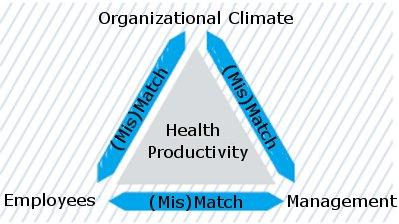
\includegraphics[natwidth=150, natheight=100]{fig1.jpg}
    \caption{Project Demopass}\label{fig:fig1}
   \end{center}
\end{figure}
%insert figure

%insert figure

%insert figure

%insert figure
%insert figure
%insert figure

Secondly, we investigated whether the two blood coagulation markers fibrinogen and D-dimer are associated with vital exhaustion (VE), a known psychosocial risk factor for coronary artery disease (CAD). Meta-analyses have established elevated fibrinogen as well as D-dimer levels in circulation as biological risk factors for the development and progression of CAD. We measured plasma fibrinogen and D-dimer concentrations in 150 apparently healthy middle-aged male and female teachers (see Kudielka et al., 2008). Linear regression yielded a significant association between vital exhaustion and fibrinogen, but not between exhaustion and D-dimer (controlling for relevant covariates). Further investigation of possible interaction effects resulted in a significant association between fibrinogen and 'VE by gender'. In secondary analyses, we therefore reran linear regression models separately for males and females. The gender-specific results revealed that the association between fibrinogen and vital exhaustion remained significant in males but not in females. This finding supports the notion that fibrinogen levels are positively related to vital exhaustion. We speculate that elevated fibrinogen might be one biological mechanism by which chronic work stress may impact on teachers' cardiovascular health in the long run. 
In a next step, we investigated the relationship between immunological factors and exhaustion in terms of burnout (see von K�nel et al., 2008a). The burnout syndrome has been previously associated with an increased risk of CAD, but the physiological mechanisms that could explain this link are still poorly understood. Knowing that a state of chronic low-grade systemic inflammation contributes to atherosclerosis, we investigated whether circulating levels of pro- and anti-inflammatory cytokines are related to burnout symptoms. For this analysis, data from 167 schoolteachers (range 23-63 years, median 48 years, 67\% women) were available; all had completed the Maslach Burnout Inventory (MBI) with its three subscales emotional exhaustion (EE), lack of accomplishment (LA), and depersonalization (DP). Levels of the proinflammatory cytokine tumor necrosis factor (TNF)-? and of the anti-inflammatory cytokines interleukin-4 and interleukin-10 (IL-4 and IL-10) were determined using fasting morning plasma samples. We computed ratios of TNF- /IL-4 and TNF-?/IL-10 as two indices of increased inflammatory activity. Analyses were adjusted for demographic factors, medication, lifestyle factors (including sleep quality), metabolic factors, and symptoms of depression and anxiety. We could demonstrate that after aggregating the three MBI subscales, higher levels of total burnout symptoms independently predicted higher TNF-? levels, lower IL-4 levels, and a higher TNF-?/IL-4 ratio. Higher levels of LA predicted decreased IL-4 levels and a higher TNF-?/IL-4 ratio. The categorical dimensions of the various burnout scales, however, did not show an independent relationship with any cytokine measure. In sum, our findings suggest an association between burnout and increased systemic inflammation along a continuum of symptom severity rather than in a categorical dimension. These results provide one explanation for the increased atherosclerotic risk observed in individuals with high levels on burnout.
It is known from epidemiological studies that chronic work stress or unfavorable work conditions are prospectively associated with different adverse health outcomes. So, in a subsequent composite analysis we investigated the relationship between chronic work stress, exhaustion and allostatic load (AL; an estimate of cumulative physiological wear-and-tear). AL could be a possible biological pathway explaining how chronic work stress or exhaustion leads to health impairments in the long run (see Bellingrath et al., in press-b). Chronic stress at work was assessed in 104 healthy female schoolteachers in terms of effort-reward-imbalance (ERI) and the extent of exhaustion (MBI, VE). Allostatic load (AL) was first analyzed according to McEwen's classical model, comprised of ten parameters including: urinary cortisol, epinephrine and norepinephrine, dehydroepiandrosterone-sulfate (DHEA-S), waist/hip ratio (WHR), glycosylated haemoglobin (HbA1c), high density lipoprotein (HDL), total cholesterol/HDL ratio, as well as systolic and diastolic blood pressure. We extended the original AL score by tumor-necrosis factor-? (TNF-?), C-reactive protein (CRP), fibrinogen, D-dimer, percent-body-fat, triglycerides and glucose. Results showed that AL scores were significantly higher in women high on effort-reward-imbalance and exhaustion (see Fig. 2). In sum, chronic work stress appears to be associated with changes in a multisystem summary indicator of physiological risk, even though participants have been in good health.



%insert figure
%insert figure
%insert figure
%insert figure
%insert figure
%insert figure
%insert figure

%insert figure




In an ongoing part of the project, we assessed physiological responses to repeated exposure to the Trier Social Stress Test (TSST) in regularly working teachers high and low on burnout and vital exhaustion (MBI, VE). We re-invited 53 medication-free, non-smoking, and healthy teachers from the initial sample (62\% of women; mean age 49.9 $\pm$ 8.58) in order to examine physiological responses to acute psychosocial stress in relation to chronic stress. Beside blood coagulation and immune measures (see von K�nel et al., revised version submitted; von K�nel et al., submitted), ACTH (5 samples), total plasma (6 samples), and free salivary cortisol (8 samples) were repeatedly measured before and after challenge (see Bellingrath et al., in press-a). In the total group, effort-reward-imbalance (ERI) and overcommitment (OC) were only marginally associated with HPA-axis responses to acute stress. However, in the subgroup of responders (N=30), high levels of OC were significantly associated with lower ACTH (p=.03), plasma (p=.02) and salivary cortisol (p<.001) responses (see Fig. 3). These results remained significant when controlling for depressive symptoms. When additionally controlling for acute perceived stressfulness of the TSST, significant associations between OC and HPA-axis responses emerged in responders as well as the total study sample. Higher levels of ERI were solely related to significantly stronger plasma cortisol increases after TSST exposure, and this effect became non-significant after controlling for depression. So far, these data support the notion of HPA-axis hyporeactivity in highly overcommitted schoolteachers. 



%insert pic
%insert pic
%insert pic
%insert pic
%insert pic
%insert pic
%insert pic
%insert pic
%insert pic
%insert pic


Results regarding longitudinal changes in depressive symptoms and plasma fibrinogen levels are reported by von K�nel et al. (in press-a). Currently, we assess HPA axis stress responses in clinically diagnosed teachers during a clinical stay. We further plan to investigate the responses of student teachers to the TSST as well as to real life stress (e.g. graded demonstration or examination lesson) in relation to work stress and burnout. 
To conclude, the Teacher Stress Study integrates different approaches and research tools from work psychology, health psychology, psychosomatic medicine and psychoneuroendocrinology into the field of "stress at work". We are convinced that a psychobiological perspective may significantly contribute to an understanding of how chronic work stress and its consequences relate to health problems.


\subsubsection{Projects/Grants}





\subsubsection{Collaborators}

\begin{itemize}
\item von K�nel Roland, Prof., MD, Head Psychosomatic Division, Department of General Internal Medicine, University Hospital / Inselspital, Bern, Switzerland
\item Hellhammer Dirk H., Prof., PhD, Department of Clinical and Physiological Psychology, University of Trier, Trier, Germany
\item W�st Stefan, PD, PhD, Deputy Research Director, Department of Genetic Epidemiology in Psychiatry, Central Institute of Mental Health, Mannheim, Germany
\item Hillert Andreas, PD, PhD MD, Medizinisch-Psychosomatische Klinik Roseneck, Prien am Chiemsee, Germany
\item Wolf Oliver T., Prof., PhD, Department of Cognitive Psychology, Ruhr-University Bochum, Bochum, Germany
\item Schlotz Wolff, PhD, School of Psychology, University of Southampton \& MRC Epidemiology Resource Centre, University of Southampton, Southampton General Hospital, UK
\item Adam Emma K., Prof., PhD, School of Education and Social Policy and Cells to Society Center, Institute for Policy Research, Northwestern University, Evanston, USA
\item Cacioppo John T., Prof., PhD, Tiffany \& Margaret Blake Distinguished Service Professor and Director, Center for Cognitive and Social Neuroscience, University of Chicago, Chicago, USA
\item Fischbach Andrea, Prof., PhD, Head of Department, Social-, Work- and Organizational Psychology, German Police University, M�nster, Germany
\item Fischer Joachim E., Prof., MD MSc, Director, Public Health, Social- and Preventive Medicine, Mannheim Institute of Public Health, Mannheim Medical Faculty, University of Heidelberg, Mannheim, Germany
\item Kirschbaum Clemens, Prof., PhD, Department of Psychology, Biological Psychology, Technical University of Dresden, Dresden, Germany
\item IRTG International Research Training Group ('Internationales Graduiertenkolleg') of Trier (Germany; Spokesmen Prof. Dr. Hartmut Sch�chinger) and Leiden (The Netherlands; Spokeswomen: Prof. Dr. Melly Oitzl)
\end{itemize}



\subsubsection{Other Professional Activities}

\textbf{Ad-hoc Reviewer}

\paragraph{Journals:}
Anxiety, Stress, \& Coping; Applied Psychology; Annals of Behavioral Medicine; Biological Psychiatry; Biological Psychology; Chronobiology International; European Journal of Oral Sciences; Frontiers in Behavioural Neuroscience (Review Editor); Health Psychology; Heart; International Archives of Occupational and Environmental Health; International Journal of Behavioral Medicine; International Journal of Cardiology; Journal of Affective Disorders; Journal of Behavioral Medicine; Journal of Clinical Endocrinology and Metabolism; Journal of Psychosomatic Research; Physiology \& Behavior; Psychiatry Research; Psychology, Health \& Medicine; Psychoneuroendocrinology; Psychophysiology; Psychosomatic Medicine; Psychosomatics; Psychotherapy and Psychosomatics; Social Science \& Medicine; Spanish Journal of Psychology; Stress; Zeitschrift f�r Arbeits- und Organisationspsychologie

\paragraph{Research Foundations:}
German Research Foundation (DFG); British Medical Research Council (MRC); The Netherlands Organisation for Health Research \& Development (ZonMw); New Zealand Foundation for Research, Science \& Technology (FRST)


\subsubsection{Publications}





%
%
%
